%%%%%%%%%%%%%%%%%%%%%%%%%%%%%%%%%%%%%%%%%%%%%%%%%%%%%%%%%%%%%%%%%%%%%%%%%%%%%%%
%                       CARREGA DE LA CLASSE DE DOCUMENT                      %
%                                                                             %
% Les opcions admissibles son:                                                %
%      12pt / 11pt            (cos dels tipus de lletra; no feu servir 10pt)  %
%                                                                             %
% catalan/spanish/english     (llengua principal del treball)                 %
%                                                                             % 
% french/italian/german...    (si necessiteu fer servir alguna altra llengua) %
%                                                                             %
% listoffigures               (El document inclou un Index de figures)        %
% listoftables                (El document inclou un Index de taules)         %
% listofquadres               (El document inclou un Index de quadres)        %
% listofalgorithms            (El document inclou un Index d'algorismes)      %
%                                                                             %
%%%%%%%%%%%%%%%%%%%%%%%%%%%%%%%%%%%%%%%%%%%%%%%%%%%%%%%%%%%%%%%%%%%%%%%%%%%%%%%

\documentclass[11pt,spanish,listoffigures,listoftables]{tfgetsinf}

%%%%%%%%%%%%%%%%%%%%%%%%%%%%%%%%%%%%%%%%%%%%%%%%%%%%%%%%%%%%%%%%%%%%%%%%%%%%%%%
%                     CODIFICACIO DEL FITXER FONT                             %
%                                                                             %
%    windows fa servir normalment 'ansinew'                                   %
%    amb linux es possible que siga 'latin1' o 'latin9'                       %
%    Pero el mes recomanable es fer servir utf8 (unicode 8)                   %
%                                          (si el vostre editor ho permet)    % 
%%%%%%%%%%%%%%%%%%%%%%%%%%%%%%%%%%%%%%%%%%%%%%%%%%%%%%%%%%%%%%%%%%%%%%%%%%%%%%%

\usepackage[T1]{fontenc}
\usepackage[utf8]{inputenc} 
\usepackage{graphicx}
\usepackage{float}
\usepackage{adjustbox}
\usepackage{textcomp}   % Maneja comillas
\usepackage{lmodern}    % Fuente moderna
\usepackage{listings}   % Para mostrar código (opcional)
\usepackage{amsmath}    % Por si hay matemáticas




%%%%%%%%%%%%%%%%%%%%%%%%%%%%%%%%%%%%%%%%%%%%%%%%%%%%%%%%%%%%%%%%%%%%%
% Para conseguir que la tabla de contenido no salga en rojo
%%%%%%%%%%%%%%%%%%%%%%%%%%%%%%%%%%%%%%%%%%%%%%%%%%%%%%%%%%%%%%%%%%%%%

\hypersetup{ colorlinks=true, linkcolor=black, urlcolor=cyan, }

%%%%%%%%%%%%%%%%%%%%%%%%%%%%%%%%%%%%%%%%%%%%%%%%%%%%%%%%%%%%%%%%%%%%%%%%%%%%%%%
%                        ALTRES PAQUETS I DEFINICIONS                         %
%                                                                             %
% Carregueu aci els paquets que necessiteu i declareu les comandes i entorns  %
%                                          (aquesta seccio pot ser buida)     %
%%%%%%%%%%%%%%%%%%%%%%%%%%%%%%%%%%%%%%%%%%%%%%%%%%%%%%%%%%%%%%%%%%%%%%%%%%%%%%%



%%%%%%%%%%%%%%%%%%%%%%%%%%%%%%%%%%%%%%%%%%%%%%%%%%%%%%%%%%%%%%%%%%%%%%%%%%%%%%%
%                        DADES DEL TREBALL                                    %
%                                                                             %
% titol, alumne, tutor i curs academic                                        %
%%%%%%%%%%%%%%%%%%%%%%%%%%%%%%%%%%%%%%%%%%%%%%%%%%%%%%%%%%%%%%%%%%%%%%%%%%%%%%%

\title{Diseño e implementación de herramientas de análisis de genoma basadas en la Teoría de la Tnformación}
\author{Cristina Rodríguez Fernández}
\tutor{Jose María Sempere Luna}
\curs{2024-2025}

%%%%%%%%%%%%%%%%%%%%%%%%%%%%%%%%%%%%%%%%%%%%%%%%%%%%%%%%%%%%%%%%%%%%%%%%%%%%%%%
%                     PARAULES CLAU/PALABRAS CLAVE/KEY WORDS                  %
%                                                                             %
% Independentment de la llengua del treball, s'hi han d'incloure              %
% les paraules clau i el resum en els tres idiomes                            %
%%%%%%%%%%%%%%%%%%%%%%%%%%%%%%%%%%%%%%%%%%%%%%%%%%%%%%%%%%%%%%%%%%%%%%%%%%%%%%%

\keywords{retinosi pigmentària, dades genòmiques, Teoria de la informació, cadenes de Markov, predicció de mutacions, machine learning, entropia}           % Paraules clau
         {retinosis pigmentaria, datos genómicos, Teoría de la información, cadenas de Markov, predicción de mutaciones, machine learning, entropía}        % Palabras clave  
         {retinitis pigmentosa, genomic data, Information Theory, Markov chains, mutation prediction, machine learning, entropy}                            % Key words

%%%%%%%%%%%%%%%%%%%%%%%%%%%%%%%%%%%%%%%%%%%%%%%%%%%%%%%%%%%%%%%%%%%%%%%%%%%%%%%
%                              INICI DEL DOCUMENT                             %
%%%%%%%%%%%%%%%%%%%%%%%%%%%%%%%%%%%%%%%%%%%%%%%%%%%%%%%%%%%%%%%%%%%%%%%%%%%%%%%

\begin{document}

%%%%%%%%%%%%%%%%%%%%%%%%%%%%%%%%%%%%%%%%%%%%%%%%%%%%%%%%%%%%%%%%%%%%%%%%%%%%%%%
%              RESUMEN DEL TFG EN CASTELLANO, VALENCIA I ANGLES                %
%%%%%%%%%%%%%%%%%%%%%%%%%%%%%%%%%%%%%%%%%%%%%%%%%%%%%%%%%%%%%%%%%%%%%%%%%%%%%%%

\begin{abstract}[spanish]
   La retinosis pigmentaria (RP), una de las distrofias hereditarias de retina (DHR) más frecuente, es conocida por una degradación progresiva en los fotorreceptores que termina por causar pérdida visual irreversible. Aún con los recientes avances en la secuenciación del genoma humano, el origen de esta condición sigue siendo un desafío debido a la amplia diversidad genética involucrada y la cantidad de genes relacionados con las DHR.

   Este Trabajo de Fin de Grado, continuación del Trabajo de Fin de Máster de Andrea Vañó Ribelles y el Trabajo de Fin de Grado de Luis Alberto Martínez Bravo, explora el uso de herramientas de Teoría de la Información y modelos de Fuentes de Markov para analizar el genoma humano, con el objetivo de predecir posibles mutaciones asociadas a la RP. Puesto que la RP es una enfermedad rara y el número de personas afectadas es muy pequeño, las técnicas de Machine Learning no resultan lo suficientemente efectivas debido a la falta de datos para desarrollar modelos robustos.

   En vez de ello, este enfoque se centra en el análisis de regiones genómicas con elevada entropía y densidad de mutaciones, ya que estas áreas serían clave para detectar variantes con mayor probabilidad de estar vinculadas a la enfermedad.

   Para ello, se han empleado los datos genómicos del National Center for Biotechnology Information (NCBI) y archivos VCF proporcionados por el Grupo de Investigación del IIS La Fe de Biomedicina Molecular, Celular y Genómica. El propósito del estudio es profundizar en las características del genoma asociadas a la enfermedad y aportar nuevas maneras de optimizar el diagnóstico genético de la retinosis pigmentaria.
   \\
   \\
\end{abstract}
\begin{abstract}[catalan]
   La retinosi pigmentària (RP) és una de les distròfies hereditàries de retina (DHR) més comunes. Es caracteritza per una degeneració progressiva dels fotoreceptors que provoca una pèrdua de visió irreversible. Malgrat els avanços en la seqüenciació del genoma humà, l'origen d'aquesta malaltia continua sent incert a causa de la gran heterogeneïtat genètica de la patologia i la quantitat de gens associats a les DHR.

   En aquest Treball de Fi de Grau, que amplia el Treball de Fi de Màster d'Andrea Vañó Ribelles i Luis, es proposa la utilització d'eines de la Teoria de la Informació i models de Fonts de Markov per a l'anàlisi del genoma humà amb l'objectiu de predir possibles mutacions associades a la RP. Com que la RP és una malaltia rara i el nombre de persones afectades és reduït, les tècniques de machine learning no resulten prou efectives a causa de l'escassetat de dades per a entrenar models robustos. En lloc d’això, aquest enfocament se centra en l’anàlisi de regions genòmiques amb alta entropia i elevada densitat de mutacions, ja que aquestes zones poden ser clau per a identificar variants amb una major probabilitat d’estar relacionades amb la patologia.

   Per a dur a terme aquest estudi, s'utilitzaran dades genòmiques disponibles al National Center for Biotechnology Information (NCBI) i arxius VCF proporcionats pel Grup d'Investigació de l'IIS La Fe de Biomedicina Molecular, Cel·lular i Genòmica. L'objectiu d'aquest treball és aprofundir en el coneixement de les característiques del genoma associades a la malaltia i aportar noves estratègies que ajuden a optimitzar el diagnòstic genètic de la retinosi pigmentària.
   \\
   \\
\end{abstract}
\begin{abstract}[english]
   Retinitis pigmentosa (RP) is one of the most common hereditary retinal dystrophies (HRD). It is characterized by the progressive degeneration of photoreceptors, leading to irreversible vision loss. Despite advances in human genome sequencing, the origin of this condition remains uncertain due to the high genetic heterogeneity of the disease and the large number of genes associated with HRD.

   In this Bachelor's Thesis, which expands upon the Master's Thesis by Andrea Vañó Ribelles and Luis, the use of Information Theory tools and Markov Source models is proposed for the analysis of the human genome, with the aim of predicting possible mutations associated with RP. Since RP is a rare disease and the number of affected individuals is limited, machine learning techniques are not sufficiently effective due to the lack of data needed to train robust models. Instead, this approach focuses on the analysis of genomic regions with high entropy and a high density of mutations, as these areas may be key to identifying variants with a higher probability of being related to the pathology.

   To achieve this, genomic data available from the National Center for Biotechnology Information (NCBI) and VCF files provided by the Research Group of the IIS La Fe in Molecular, Cellular and Genomic Biomedicine will be used. The purpose of this study is to deepen the understanding of the genomic features associated with the disease and to provide new strategies that help optimize the genetic diagnosis of retinitis pigmentosa.
   \\
   \\
\end{abstract}

%%%%%%%%%%%%%%%%%%%%%%%%%%%%%%%%%%%%%%%%%%%%%%%%%%%%%%%%%%%%%%%%%%%%%%%%%%%%%%%
%                              CONTINGUT DEL TREBALL                          %
%%%%%%%%%%%%%%%%%%%%%%%%%%%%%%%%%%%%%%%%%%%%%%%%%%%%%%%%%%%%%%%%%%%%%%%%%%%%%%%

\mainmatter

%%%%%%%%%%%%%%%%%%%%%%%%%%%%%%%%%%%%%%%%%%%%%%%%%%%%%%%%%%%%%%%%%%%%%%%%%%%%%%%
%                                 INTRODUCCION                                %
%%%%%%%%%%%%%%%%%%%%%%%%%%%%%%%%%%%%%%%%%%%%%%%%%%%%%%%%%%%%%%%%%%%%%%%%%%%%%%%

\chapter{Introducción}

La retinosis o retinitis pigmentaria (RP), una de las distrofias hereditarias de retina DHR más frecuente, es un grupo de enfermedades conocidas por una degradación progresiva en los fotorreceptores (células de la retina responsables de captar la luz y, por tanto, permitir la visión) que termina por causar pérdida visual irreversible. Esta patología suele manifestarse en un principio con ceguera nocturna, seguida por una reducción del campo visual periférico y, en fases avanzadas, puede llegar a la pérdida de la visión central\cite{NAT}. La RP presenta una gran heterogeneidad genética, lo que significa que puede estar causada por mutaciones en más de 100 genes diferentes, heredados bajo distintos patrones\cite{GIL}. Aún con los recientes avances en la secuenciación del genoma humano, el origen de esta condición sigue siendo un desafío debido a la amplia diversidad genética involucrada y la cantidad de genes relacionados con las DHR. 

\begin{figure}[H]
   \centering
   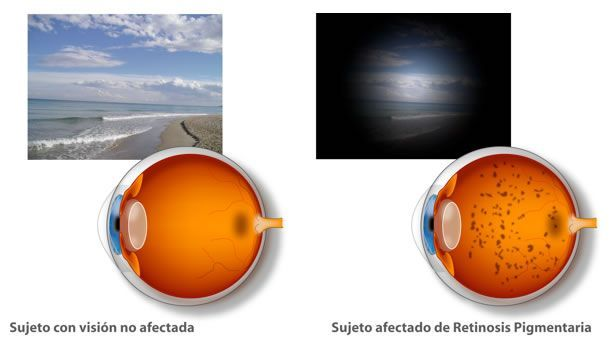
\includegraphics[width=0.9\textwidth]{Retinosis-Pigmetaria.jpg}
   \caption{Ejemplo de visión de un paciente con visión normal y un paciente con RP.}
   \label{fig:etiqueta_opcional2}
\end{figure}

Este Trabajo de Fin de Grado, continuación del Trabajo de Fin de Máster de Andrea Vañó Ribelles y el Trabajo de Fin de Grado de Luis Alberto Martínez Bravo, explora el uso de herramientas de Teoría de la Información y modelos de Fuentes de Markov para analizar el genoma humano, con el objetivo de predecir posibles mutaciones asociadas a la RP. Puesto que la RP es una enfermedad rara y el número de personas afectadas es muy pequeño, las técnicas de Machine Learning no resultan lo suficientemente efectivas debido a la falta de datos para desarrollar modelos robustos. 

 

En vez de ello, este enfoque se centra en el análisis de regiones genómicas con elevada entropía y densidad de mutaciones, ya que estas áreas serían clave para detectar variantes con mayor probabilidad de estar vinculadas a la enfermedad. 

 

Para ello, se han empleado los datos genómicos del National Center for Biotechnology Information (NCBI) y archivos VCF proporcionados por el Grupo de Investigación del IIS La Fe de Biomedicina Molecular, Celular y Genómica. El propósito del estudio es profundizar en las características del genoma asociadas a la enfermedad y aportar nuevas maneras de optimizar el diagnóstico genético de la retinosis pigmentaria. 

\section{Motivación}

\subsection{Motivación personal}
Desde que comencé mi formación en Ingeniería Informática, siempre he tenido la convicción de que esta no debe limitarse a aspectos técnicos, algoritmos o eficiencia computacional, sino que debe orientarse también hacia herramientas que tengan un impacto positivo en la vida de las personas. Por eso, me interesan especialmente las aplicaciones la Inteligencia Artificial para mejorar la sociedad, hacer el mundo más justo e inclusivo y resolver problemas reales.  

Siguiendo estos objetivos, y gracias al proyecto conjunto del Instituto VRAIN con el Grupo de Investigación del IIS La Fe de Biomedicina Molecular, Celular y Genómica, he tenido la oportunidad de formarme en diversas áreas de conocimiento y aplicar mis conocimientos técnicos a una dimensión ética y social. Por esta razón, considero que mejorar la calidad de vida de pacientes mediante herramientas que ayuden a investigadores y personal sanitario en el diagnóstico es una de las principales motivaciones que me impulsa en la realización de este proyecto. 

\subsection{Motivación profesional}
Las distrofias hereditarias de retina (DHR) constituyen un conjunto de enfermedades genéticas que afectan a la estructura y función de la retina, llevando progresivamente a la pérdida de visión, en muchos casos hasta alcanzar la ceguera legal. A pesar de ser consideradas enfermedades raras, su impacto es profundo y duradero, no solo desde el punto de vista funcional, sino también psicológico, afectando significativamente la calidad de vida de quienes las padecen\cite{STO}.

Actualmente, no existe ningún tratamiento curativo, aunque se están explorando alternativas terapéuticas como las que se describen en la sección 2 de esta memoria, pero aún se encuentran en fase experimental. En este contexto, el diagnóstico genético tiene un papel fundamental en la orientación médica y la inclusión del paciente en ensayos clínicos\cite{HAN}.

Uno de los principales desafíos en el estudio genético de las distrofias hereditarias de retina (DHR) radica en la gestión y análisis de la enorme cantidad de variantes obtenidas a partir de técnicas como la secuenciación del exoma completo (WES). Aunque se aplican filtros por frecuencia poblacional o predictores del impacto funcional, el volumen de información sigue siendo elevado, lo que dificulta alcanzar un diagnóstico genético preciso\cite{DEC}.

En este trabajo se propone un enfoque complementario, basado en el uso de modelos computacionales que aplican principios de la teoría de la información y fuentes de Markov para analizar la secuencia genómica antes y después de la introducción de mutaciones. A través de métricas como la entropía y la densidad mutacional, se busca detectar alteraciones estructurales o funcionales que puedan asociarse con variantes patológicas. Esta estrategia no solo contribuye al desarrollo de nuevas herramientas de apoyo al diagnóstico, sino que también tiene una dimensión humana relevante: mejorar el acceso a un diagnóstico certero, lo que representa un paso fundamental para que los pacientes y sus familias encuentren respuestas, orientación clínica y esperanza de acceso a futuras terapias. 

\section{Objetivos}

El objetivo principal de este Trabajo de Fin de Grado es proporcionar herramientas informáticas para el análisis genómico, en concreto aplicado a enfermedades raras como la Retinosis Pigmentaria (RP). Para ello contamos con archivos que contienen información sobre mutaciones y secuencias completas del genoma, y se implementan modelos basados en Teoría de la Información y Fuentes de Markov, con el fin de identificar regiones genómicas relevantes y predecir mutaciones potencialmente patogénicas.

\subsection{Procesamiento de archivos VCF y secuencias genómicas}

Hacer uso de herramientas y librerías de uso biomédico que permitan la lectura, escritura y análisis de archivos genéticos, y de esta manera, realizar un preproceso y de la información genética y aplicar mutaciones sobre la secuencia de referencia de forma precisa y eficiente.

Preguntas de Investigación: 
\begin{itemize}
\item ¿Qué formato presentan los archivos VCF y cómo se puede garantizar la compatibilidad con los archivos FASTA con la secuencia genómica?
\item ¿Cómo se pueden integrar las trasformaciones necesarias en la secuencia de referencia de manera correcta y sin conflictos entre ellas?
\end{itemize}

\subsection{Aplicación de Teoría de la Información y Fuentes de Markov al análisis de secuencias genómicas }

Utilizar modelos de Teoría de la Información y Fuentes de Markov para predecir el impacto de las mutaciones en la secuencia genómica y así detectar zonas con valores anómalos de entropía, o alta densidad de mutaciones, para su posterior estudio. 

Preguntas de Investigación: 
\begin{itemize}
\item ¿Qué diferencias se observan en los valores de entropía, tanto la simple como la realizada a partir de aplicar Fuentes de Markov, entre la secuencia original y la mutada? 
\item ¿Hay alguna correlación entre las zonas con alta densidad de mutaciones y los valores de entropía? 
\item ¿Cómo es la estructura que presenta el autómata de transición generado a partir de Fuentes de Markov de orden k? 
\item ¿Cuáles son los valores óptimos de los parámetros para obtener resultados interesantes? 
\end{itemize}

\subsection{Desarrollo de una interfaz de usuario para la visualización de resultados }

Crear una aplicación para facilitar el uso del programa, sin necesidad de tener conocimientos avanzados en informática. Esto es especialmente importante en este contexto, ya que se trata de una herramienta enfocada a un usuario que no es experto en informática. Además, esta interfaz debe permitir la interacción del usuario con la aplicación, modificando distintos parámetros para obtener diferentes resultados en función de lo que se busque, y visualizar gráficamente y de manera unificada los resultados de este análisis. 

Preguntas de Investigación: 
\begin{itemize}
\item ¿Qué diseño debe tener la interfaz para que no sea demasiado compleja, pero permita interactuar ampliamente al usuario? 
\item ¿Cómo presentar los resultados de manera ordenada, clara y concisa, para hacer accesible la información más complicada? 
\end{itemize}

\subsection{Contribución a las aplicaciones de la IA en el campo de la investigación genética }

Proponer un nuevo enfoque de análisis genómico basado en la Teoría de la Información, el cual no se había estudiado aún, y ofrecer una herramienta efectiva para el estudio de otras enfermedades raras con componente genético. 

Preguntas de Investigación: 
\begin{itemize}
\item ¿Debe poder generalizarse el proyecto para otras patologías? 
\item ¿Qué técnicas se podrían utilizar sobre los resultados obtenidos, como machine learning, para clasificar o encontrar patrones de mutaciones? 
\end{itemize}


\section{Estructura de la memoria}

La memoria de este TFG está estructurada en 7 secciones, cada una de estas a su vez divididas en subsecciones.  


La primera sección se introduce el proyecto, se exponen el contexto y la motivación, y se justifican los objetivos. En la sección 2, se realiza una investigación del conocimiento y tecnologías existentes en la actualidad sobre el tema que se aborda en el proyecto, así como las limitaciones que aún existen, lo que justifica la necesidad de este proyecto. En la sección 3, se realiza una exposición de los conceptos clave necesarios para entender este trabajo, genética y mutaciones, los archivos genómicos utilizados y los principios de la Teoría de la Información. Después, en la sección 4, se describe la metodología seguida y el flujo de información y herramientas usadas a lo largo del proyecto. En la sección 5, se explica detalladamente el funcionamiento del programa. En la sección 6 se exponen y analizan los resultados obtenidos mediante la realización de pruebas cambiando los diferentes parámetros. Por último, en la sección 7, se finaliza el trabajo, explicando las conclusiones obtenidas, seguida por un listado de las referencias bibliográficas utilizadas. 


%\section{Notes bibliografiques} %%%%% Opcional

%????? ????????????? ????????????? ????????????? ????????????? ?????????????

%%%%%%%%%%%%%%%%%%%%%%%%%%%%%%%%%%%%%%%%%%%%%%%%%%%%%%%%%%%%%%%%%%%%%%%%%%%%%%%
%                                ESTADO DEL ARTE                              %
%%%%%%%%%%%%%%%%%%%%%%%%%%%%%%%%%%%%%%%%%%%%%%%%%%%%%%%%%%%%%%%%%%%%%%%%%%%%%%%

\chapter{Estado del arte}

El campo del análisis genómico de la retinosis pigmentaria (RP) está avanzando rápidamente, con desarrollos en la identificación genética, herramientas de predicción y terapias emergentes. Sin embargo, en un contexto de disponibilidad limitada de especialistas en retina, pruebas y asesoramiento genético, sigue existiendo una gran necesidad de métodos diagnósticos precisos y accesibles. Esta situación ha motivado la búsqueda de nuevas técnicas para mejorar la detección de esta enfermedad.

\section{Métodos tradicionales}

Los métodos tradicionales basados en sistemas de codificación médica como el ICD (International Classification of Diseases) y el SNOMED (Systematized Nomenclature of Medicine) han sido ampliamente utilizados en la medicina para clasificar enfermedades y registrar diagnósticos. Sin embargo, en el caso de enfermedades genéticas raras como la retinosis pigmentaria (RP), estos sistemas de codificación presentan importantes limitaciones\cite{VER}. Esto es debido a que es una patología altamente heterogénea a nivel genético y clínico: existen numerosas mutaciones responsables y los síntomas pueden evolucionar de formas muy diversas entre pacientes\cite{HAR}. 

Debido a esta complejidad, se ha recurrido a técnicas más especificas como los paneles genéticos dirigidos o la secuenciación de exoma completo (WES). Estos enfoques son capaces de examinar una gran cantidad de mutaciones de cada paciente. No obstante, muchos pacientes quedan sin un diagnositco definitivo debido a la dificultad para interpretar el gran volumen de información relativa a las variantes encontradas tras la secuenciación.

\section{Inteligencia Artificial}

En la actualidad se están utilizando métodos basados en inteligencia artificial (IA) para la detección, diagnóstico y pronóstico de numerosas enfermedades en distintas áreas de la medicina, desde oncología hasta neurología o cardiología. Esto es debido a la capacidad de la IA para trabajar con grandes volúmenes de datos e identificar en estos patrones complejos para generar predicciones con una alta precisión\cite{FER}. No obstante, su desarrollo para las distrofias hereditarias de retina (DHR), específicamente la retinosis pigmentaria (RP) todavía está en una fase temprana.

\subsection{Aplicaciones de Machine Learning}

El aprendizaje profundo (deep learning) es una subcategoría de la inteligencia artificial que ha ganado mucha atención en los últimos años, especialmente porque el aprendizaje profundo es muy eficaz en el reconocimiento de patrones y el análisis de imágenes\cite{STE}.

Inspirado en el cerebro humano, el aprendizaje profundo (Deep Learning) ha sido desarrollado utilizando redes neuronales para aprender a partir de datos, extrayendo y comprendiendo automáticamente características complejas. Un ejemplo común del uso del aprendizaje profundo en imágenes médicas son las redes neuronales convolucionales (CNN, por sus siglas en inglés). Las CNN participan en diversas tareas relacionadas con imágenes, como la detección, el reconocimiento y la segmentación de imágenes, mediante el uso de información espacial, la detección de características locales y la reducción de la complejidad del modelo a través del muestreo, el uso compartido de pesos y los campos receptivos locales\cite{SHE}.

En un estudio reciente, se utilizaron tres modelos preentrenados; Inception-v3, ResNet-50 y VGG-19, para clasificar imágenes retinianas asociadas a diferentes genes relacionados con la retinosis pigmentaria. Tras un preprocesamiento exhaustivo que incluyó técnicas de class balancing y boosting para corregir la variabilidad genética, los modelos obtuvieron precisiones superiores al 80\% en los datos de training\cite{FER}. Sin embargo, al aplicar estos modelos a datos de testing, las tasas de precisión cayeron a un 54\%, 56\% y 54\% respectivamente, resultados claramente insuficientes para garantizar un diagnóstico clínico fiable debido a la elevada tasa de error.

Los estudios de IA disponibles, como el mencionado anteriormente, que buscan la detección, clasificación y predicción de DHR, siguen siendo en su mayoría retrospectivos e incluyen un número relativamente limitado de pacientes debido a su escasez\cite{ISS}. Esto pone de manifiesto la necesidad de continuar optimizando las metodologías empleadas para alcanzar niveles de exactitud que resulten aceptables en el ámbito médico.

\subsection{Aplicaciones de Teoría de la Información y Fuentes de Markov}

Aunque actualmente no existen estudios específicos que utilicen directamente Teoría de la Información y Fuentes de Markov al análisis genómico de la RP, estos enfoques se han consolidado como potenciales herramientas.

Sabemos que la Teoría de la Información es útil para medir la cantidad de información, la incertidumbre y el contenido informativo en sistemas complejos, como es el caso del genoma humano. En genómica, conceptos como la entropía permiten detectar mutaciones en el genoma humano, ya que son capaces de identificar cambios en la información genética, comparar con referencias conocidas o analizar patrones\cite{SEC}.

Por su parte, los modelos de Fuentes de Markov (de orden k) permiten capturar patrones de dependencia entre nucleótidos y por lo tanto identificar regiones del genoma con propiedades estadísticas anómalas\cite{VOZ}, indicativas de posibles mutaciones patológicas.

\section{Otras terapias emergentes}

Además de los enfoques basados en el análisis genético, en los últimos años también se está abordando el problema desde la estrategia de la terapia genética, un tipo de terapia curativa que busca tratar la causa subyacente de una enfermedad genética corrigiendo o reemplazando directamente el gen defectuoso. Esta va dirigida al gen RPGR que es uno de los genes del cromosoma X que comúnmente está asociado a la RP (se tiene constancia de que es el causante de entre el 70\% y el 90\% de los casos ligados al cromosoma X)\cite{WAN}. Estas terapias consisten en la inyección subretinal de un virus modificado que transporta copias funcionales del gen RPGR, con el objetivo de restaurar la función perdida en las células de la retina afectadas\cite{ZON}. Este tipo de tratamiento que se encuentra aún en fase de ensayo clínico, representa una posible cura genética para determinados subtipos de la RP, especialmente en pacientes jóvenes donde el daño celular aún no es irreversible.

Sin embargo, para que estas terapias sean verdaderamente efectivas, es esencial identificar de manera precisa las mutaciones responsables. Mediante el uso de herramientas basadas en Teoría de la Información es posible identificar de forma eficiente estas variantes, y así seleccionar a los candidatos adecuados para las terapias génicas y optimizar los ensayos clínicos.


%%%%%%%%%%%%%%%%%%%%%%%%%%%%%%%%%%%%%%%%%%%%%%%%%%%%%%%%%%%%%%%%%%%%%%%%%%%%%%%
%                         CAPITOLS (tants com calga)                          %
%%%%%%%%%%%%%%%%%%%%%%%%%%%%%%%%%%%%%%%%%%%%%%%%%%%%%%%%%%%%%%%%%%%%%%%%%%%%%%%

\chapter{Fundamentos teóricos}

\section{Conceptos básicos de genética y mutaciones}

En el núcleo de cada célula humana se encuentra el ADN, que contiene toda la información genética necesaria para el funcionamiento y desarrollo del organismo. El ADN está formado por una cadena de nucleótidos, que son las unidades básicas del material genético. Cada nucleótido se compone de tres partes: un grupo fosfato, un azúcar (desoxirribosa en el caso del ADN) y una base nitrogenada.

Las bases nitrogenadas son moléculas orgánicas que contienen nitrógeno y que se agrupan en dos tipos principales: purinas y pirimidinas. En el ADN existen cuatro bases nitrogenadas: adenina (A) y guanina (G), que son purinas; y citosina (C) y timina (T), que son pirimidinas. Estas bases se emparejan de forma complementaria (A con T y C con G), lo que permite la formación de la estructura de doble hélice característica del ADN\cite{GEN}.


\begin{figure}[H]
   \centering
   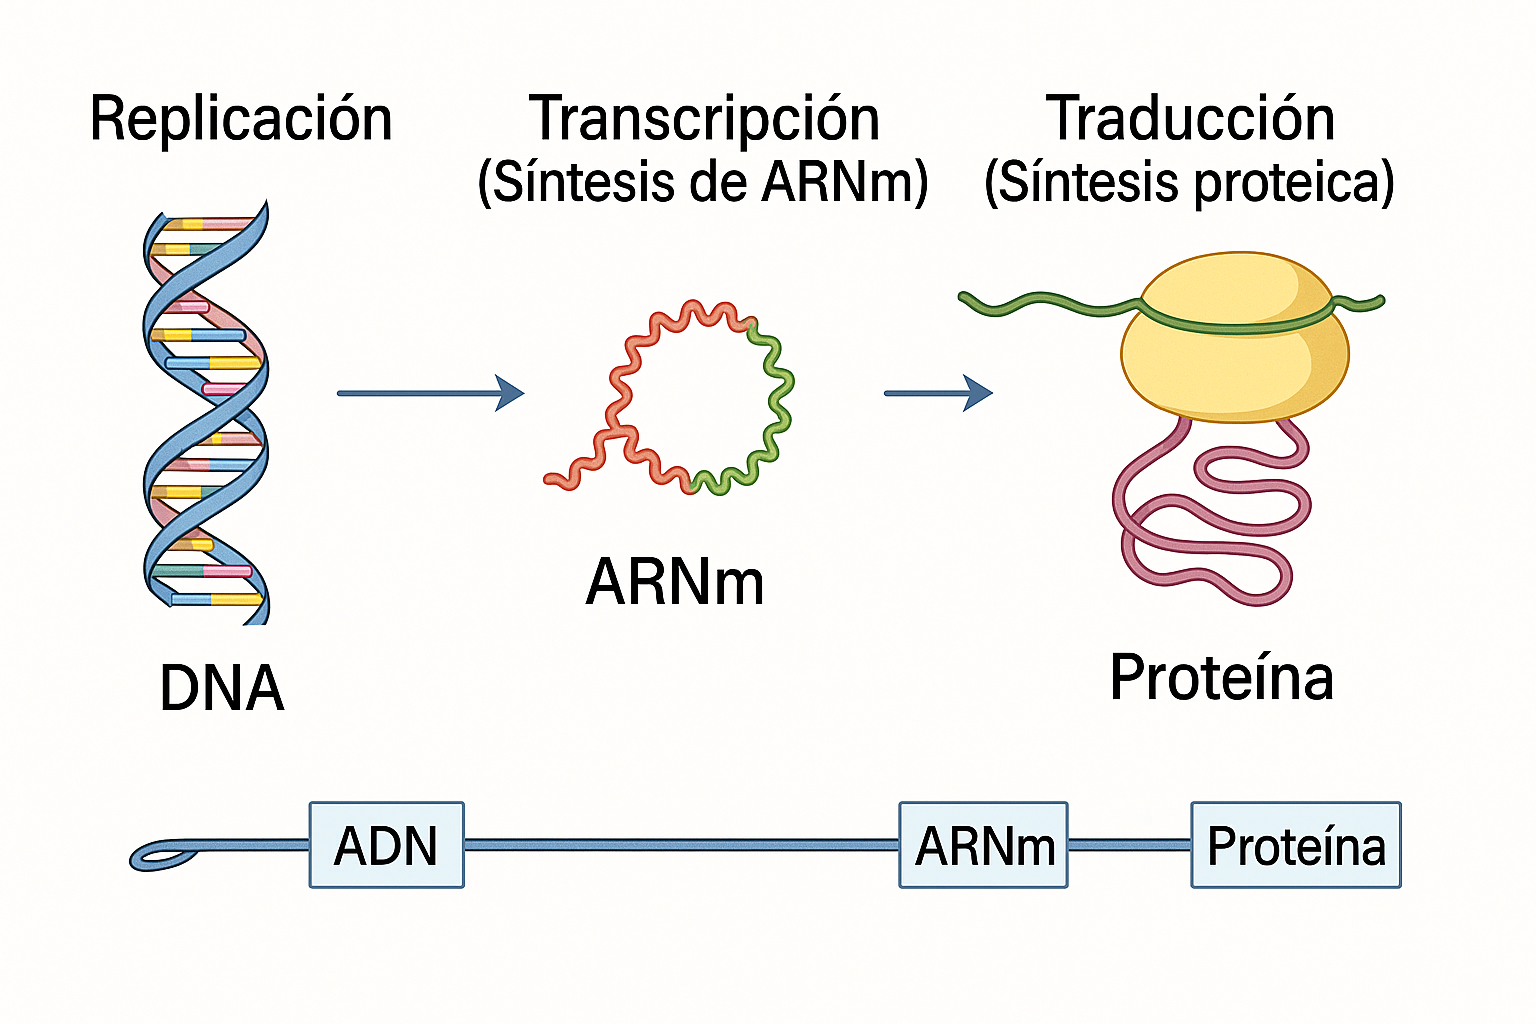
\includegraphics[width=0.9\textwidth]{ADN.png}
   \caption{Procesos genéticos de la síntesis de proteínas.}
   \label{fig:etiqueta_opcional1}
\end{figure}

Sin embargo, el ADN no actúa directamente para realizar funciones celulares. En su lugar, esa información debe ser primero transcrita en moléculas de ARN (en este la timina se sustituye por uracilo, otra pirimidina), las cuales desempeñan roles clave en la expresión génica. Este proceso, conocido como transcripción, da lugar a diferentes tipos de ARN, que luego participan en distintos mecanismos celulares.

Existen dos tipos principales de transcritos que resultan de este proceso: el ARN mensajero (ARNm), que lleva la información del ADN a los ribosomas para la síntesis de proteínas, y el ARN no codificante (ARNnc), que, aunque no se traduce en proteínas, cumple funciones esenciales como la regulación génica, la modificación del ARN, la estructura de los ribosomas y otras tareas fundamentales para el control celular\cite[p.~254-300]{WAT}. 

El ARN mensajero (ARNm) actúa como intermediario entre el ADN y las proteínas de la siguiente manera: mediante el proceso de traducción, los ribosomas convierten cada molécula de ARNm en una proteína, es decir, en una secuencia de aminoácidos. Cada proteína adopta una estructura tridimensional compleja y funciones específicas. Gracias a la interacción entre el ADN, ARN y proteínas, el genoma es capaz de regular qué células deben crecer, morir y cómo se estructuran, entre otras funciones\cite{RIN}. 


Por esta razón, cada individuo presenta un genoma ligeramente distinto al resto. Estas diferencias son conocidas como variaciones o mutaciones genómicas, y pueden suponer variaciones de un único nucleótido o múltiples nucleótidos. Estos cambios influyen en el fenotipo del individuo y también pueden ser responsables de ciertas enfermedades. 

\begin{itemize}
   \item SNV: sustitución de una sola base del ADN por otra. Es el tipo más común de variación genética en el genoma humano. 
   \begin{itemize}
      \item Sinónima: La sustitución no cambia el aminoácido codificado por el codón, debido a la degeneración del código genético. No suele tener efecto funcional, aunque puede afectar la eficiencia de traducción o el splicing. 
      \item No sinónima: Cambia el aminoácido codificado. Esta a su vez se subdivide en Missense (se sustituye un aminoácido por otro, por lo que puede alterar la función o estructura de la proteína) y Nonsense (introduce un codón de parada prematuro, truncando la proteína, y esta normalmente acaba inactiva o no funcional). 
   \end{itemize}
   
   \item  Indels (Inserciones y deleciones): Variaciones que implican la inserción o eliminación de un pequeño número de nucleótidos. Son el segundo tipo más común de variación.
   \begin{itemize}
      \item In-frame indel: El número de nucleótidos es múltiplo de 3. Esto afecta uno o más codones completos, pero no altera el marco de lectura. Puede tener o no efecto funcional. 
      \item Frameshift indel: El número de nucleótidos no es múltiplo de 3, por lo que altera el marco de lectura de todo el gen a partir del punto del indel, generando proteínas aberrantes y normalmente no funcionales. 
   \end{itemize}
   \item Copy Number Variation (CNV): Amplificaciones o deleciones de segmentos largos del ADN. Pueden incluir genes completos o regiones reguladoras. Pueden estar relacionadas con la variabilidad fenotípica, trastornos del desarrollo y enfermedades neuropsiquiátricas\cite{ZHA}.
   \item Structural Variation (SV): Alteraciones grandes en la estructura del genoma que incluyen inversiones, translocaciones, inserciones o deleciones mayores.
   \begin{itemize}
      \item Inversiones: Un segmento se invierte dentro del mismo cromosoma. 
      \item Translocaciones: Fragmentos de ADN se trasladan a otras posiciones o cromosomas.
      \item Grandes deleciones/duplicaciones: afectan múltiples genes/regiones. 
   \end{itemize}
\end{itemize}


\section{Conceptos básicos de ficheros genéticos}

Las tecnologías de secuenciación de nueva generación (NGS) son muy utilizadas hoy en día en investigación genómica y biomédica. Para facilitar el análisis y transferencia de datos, se han definido diferentes formatos de archivos estándar. 

Cuando se secuencia una muestra biológica mediante un sistema de NGS, se generan pequeños fragmentos de ADN o ARN que representan secuencias del genoma, conocidos como lecturas. Estas lecturas se almacenan en archivos de lectura cruda (raw read files). Los formatos más comunes son: fasta, fastq y fasta.gz. 

Después, esas lecturas deben ser alineadas con el genoma de referencia (como el genoma humano), y el resultado de este alineamiento se guarda en archivos SAM (Sequence Alignment Map) o BAM (Binary Alignment Map). 

Por último, a partir de los archivos de alineamiento anteriores, se pueden realizar análisis posteriores para entender la muestra:  

\begin{itemize}
   \item Si el objetivo es identificar mutaciones (como los SNV), esta información se guarda en un archivo con formato VCF (Variant Call Format) o BCF (BIinary Call Format). 
   \item Si se desea medir la densidad de lecturas en diferentes zonas del genoma, se obtienen archivos con formato Wiggle, BedGraph, BigWig o cWig.
   \item Si se busca definir regiones que estén cubiertas por lecturas (por ejemplo, para identificar exones), los resultados se almacenan en formato bed o bigBed.
\end{itemize}

En este proyecto, nos enfocaremos principalmente en dos de estos formatos: 

\subsection{FASTA}

El formato FASTA es un formato de texto estándar para representar secuencias biológicas como ADN, ARN y proteínas mediante letras. Permite incluir nombres y comentarios de las secuencias. Es simple y permite la manipulación de secuencias usando herramientas de procesamiento de texto\cite{JAV}. Un archivo FASTA consta de una o varias secuencias estructuradas de la siguiente manera: una línea de encabezado que debe comenzar con el carácter ‘>’ seguido de un identificador único de secuencia (SeqID), y la secuencia de nucleótidos que puede estar compuesta por una o varias líneas \cite{FAS}.

\begin{table}[H]
   \centering
   \caption{Ejemplo de archivo en formato FASTA}
   \begin{tabular}{|l|}
   \hline
   \texttt{>chr1\_example\_sequence} \\ \hline
   \texttt{AGCTGATCGATCGATCGTACGTAGCTAGCTGACT} \\
   \texttt{GCTAGCTAGCATCGATCGTAGCTAGCTAGCTGAC} \\
   \texttt{TAGCTAGCTAGCATCGATCGATCGATCGATCGTA} \\
   \hline
   \end{tabular}
   \label{tabla:FASTA}
   \end{table}
   

Gracias a su estructura sencilla y la compatibilidad con la mayoría de las herramientas bioinformáticas, se ha convertido en un formato estándar por su eficiencia para manipular secuencias biológicas\cite{GEN}

\subsection{VCF}

VCF es un formato de archivo de texto utilizado en bioinformática específicamente diseñado para almacenar información sobre variantes genómicas, detectadas mediante procesos de secuenciación del ADN. Se trata de un estándar utilizado en múltiples proyectos genómicos a gran escala, como es el 1000 Genome Project\cite{AUT}. Esto es debido a que se trata de un archivo muy estructurado y con capacidad de representar de manera clara y eficaz las variaciones observadas en una o varias muestras, y su facil escalabilidad\cite{EMB}.

Dado que los archivos VCF estan diseñados para albergar una gran cantidad de información, existe un formato binario alternativo llamado BCF (Binary Call Format) para facilitar su almacenamiento, transferencia y análisis computacional, ya que es una versión comprimida del anterior. 

Un archivo VCF consta de una cabecera y una sección de datos: 

\begin{itemize}
   \item La cabecera incluye un número arbitrario de líneas de metainformación, las cuales van precedidas de \texttt{\#\#}. Estas definen el contenido, las convenciones utilizadas, los tipos de anotaciones y los nombres de las columnas de la sección de datos\cite{DAN}.
      \begin{table}[H]
         \centering
         \caption{Ejemplo de cabecera de un archivo VCF}
         \begin{tabular}{|l|}
         \hline
         \texttt{\#\#fileformat=VCFv4.2} \\
         \texttt{\#\#FILTER=<ID=PASS,Description="All filters passed">} \\
         \texttt{\#\#INFO=<ID=AF,Number=A,Type=Float,Description="Allele Frequency">} \\
         \texttt{\#\#FORMAT=<ID=GT,Number=1,Type=String,Description="Genotype">} \\
         \texttt{\#CHROM POS ID REF ALT QUAL FILTER INFO FORMAT SAMPLE1 SAMPLE2} \\
         \hline
         \end{tabular}
         \label{tabla:cabeceraVCF}
      \end{table}
      
   \item En la sección de datos, cada fila corresponde a una variante identificada, de la cual se incluye la siguiente información estructurada en diferentes columnas: CHROM y POS describen el cromosoma y la posición de inicio en el genoma donde se encuentra la variante, ID es el identificador único de la variante, REF guarda cual debe ser el alelo de referencia según la base genómica establecida, ALT es la lista de alelos alternativos observados (separados por punto y coma si hubiera más de uno), QUAL es la puntuación de calidad de la variante (la confianza en esta), FILTER define el resultado del proceso de filtrado (si la variante pasa los controles de calidad), y por último INFO contiene anotaciones adicionales sobre la variante\cite{EMB}. Además, cuando el archivo VCF incluye información de varias muestras, se agregan diferentes siguientes campos entre los que destaca FORMAT, lista la cual define qué tipo de información se añade para cada muestra. 
      \begin{table}[H]
         \centering
         \caption{Ejemplo de la sección de datos en un archivo VCF}
         \begin{adjustbox}{width=\textwidth}
         \begin{tabular}{|l|r|l|l|l|r|l|l|l|l|l|}
         \hline
         \textbf{CHROM} & \textbf{POS} & \textbf{ID} & \textbf{REF} & \textbf{ALT} & \textbf{QUAL} & \textbf{FILTER} & \textbf{INFO} & \textbf{FORMAT} & \textbf{SAMPLE1} & \textbf{SAMPLE2} \\
         \hline
         3 & 879317 & rs112 & G & A & 99.0 & PASS & AF=0.5;DP=100 & GT:DP & 0/1:48 & 1/1:52 \\
         3 & 879445 & . & T & CTT & 72.5 & PASS & AF=0.25;DP=80 & GT:DP & 0/0:42 & 0/1:38 \\
         3 & 879587 & rs119 & C & T & 85.2 & PASS & AF=0.33;DP=90 & GT:DP & 1/1:45 & 0/1:45 \\
         \hline
         \end{tabular}
         \end{adjustbox}
         \label{tabla:ejemploVCF}
      \end{table}
      
      
      
\end{itemize}



\section{Teoría de la Información}

La teoría de la información es una disciplina que estudia la cuantificación, almacenamiento y comunicación de datos, especialmente enfocada en la transmisión de información a través de canales. Fue desarrollada por Claude Shannon y Warren Weaver en los años 40. Sin embargo, su aplicación se ha extendido a otros campos como la informática, la lingüística, o la biología\cite{COV}.

“Una fuente de información se define como un par (S, P) donde S es un alfabeto predefinido y P es una distribución de probabilidad sobre S. Dado que la fuente de información introduce una incertidumbre en la variable aleatoria definida por el alfabeto predefinido, la entropía mide el grado de incertidumbre de dicha variable. También el grado de aleatoriedad en la fuente de información y, en consecuencia, permite estimar las unidades de información necesarias en promedio para codificar todos los valores posibles que puedan darse en la fuente de información.”\cite{fuentesupv}

Para entender mejor esta idea, definiremos unos conceptos clave:  

\subsection{Canal de comunicación }

Un canal de comunicación es el medio físico o digital a través del cual se transmite la información.  

\subsection{Compresión de datos}

La compresión hace referencia a la reducción del tamaño de los datos sin perder información.  

\subsection{Código}

El código es el sistema de símbolos o señales utilizado para representar la información. 

\subsection{Entropía} 

El concepto de entropía se introdujo en el siglo XIX en la termodinámica como una magnitud física que media el grado de desorden en un sistema. En la etapa de 1940, Shanon trasladó este concepto al ámbito de las comunicaciones, ya que definió la entropía como una medida de incertidumbre o sorpresa asociada a un conjunto de mensajes\cite[p.~4]{ROB}. Esta idea fundó lo que se conoce hoy en día como Teoría de la Información. Dada una variable aleatoria X con distribución de probabilidad P, la entropía se define como: 

\[
H(X) = - \sum_{i=1}^{n} p(x_i) \log_2 p(x_i)
\]

La entropía se interpreta como el número promedio de bits necesarios para codificar los resultados de una variable aleatoria. 

\begin{itemize}
   \item Entropía máxima: si una variable aleatoria tiene n resultados igualmente probables, es decir, todos tienen la misma probabilidad de ocurrencia, su entropía vale log 2 n. 
   \item Entropía mínima: si hay certeza de ocurrencia de un evento, es decir, tiene probabilidad 1 y por lo tanto el resto 0, la entropía vale 0. \cite[p.~7]{ROB}
\end{itemize}
 
En el contexto de este Trabajo de Fin de Grado, esta idea se aplica a secuencias de ADN, donde cada símbolo representa una base nitrogenada (Adenina, Citosina, Timina y Guanina) y la probabilidad de ocurrencia de cada una se mide mediante la frecuencia relativa en una región determinada del genoma. Por ejemplo, calcular la entropía de un conjunto de k-mers en una secuencia de ADN podría ayudar a identificar regiones altamente conservadas o variables. Estas regiones pueden correlacionarse con funciones biológicas importantes, como promotores, regiones reguladoras, o sitios de mutación frecuentes. 

\subsection{Información}

Los conceptos de entropía e información están relacionados, pero es importante saber distinguirlos. La información es la diferencia entre la máxima entropía (por ejemplo, en una situación de incertidumbre total) y la entropía actual (con cierta cantidad de conocimiento). La información por tanto representa la reducción de incertidumbre:

\[
I(X:Y) = H(X) - H(X \mid Y)
\]

Esta relación se conoce como información mutua y cuantifica la cantidad de información que se obtiene de la variable X al conocer la variable Y. Es fundamental en muchos contextos como el análisis de datos o el análisis genómico, ya que ayuda a conocer las correlaciones entre una base y su contexto, o con otras entidades como proteínas, regiones funcionales o mutaciones. 


\subsection{Modelos de Fuentes de Markov}

“Una fuente de información con memoria nula se define como un par (S,P) donde la emisión de cada símbolo \( s_i \) sólo depende de su probabilidad \( p(s_i) \). Una fuente de información con memoria (de orden \( m \)) se define como un par (S,P) de forma que la emisión de cada símbolo \( s_i \) depende de los \( m \) símbolos emitidos con anterioridad, con una probabilidad condicional \( p(s_i \mid s_{i1}, s_{i2}, \dots, s_{im}) \).”\cite{fuentesupv}

Las fuentes de información básicas no tienen memoria, es decir, en el cálculo de la probabilidad de una determinada base no se tienen en cuenta las bases anteriores. Sin embargo, en genómica, el ADN no es del todo aleatorio, ciertas bases tienden a seguir a otras con mayor probabilidad, lo que sugiere que un modelo de Fuente de Markov puede ser más realista. 

Una Fuente de Markov (o fuente de información con memoria) se define como un sistema donde la probabilidad de que ocurra cada símbolo depende de los símbolos que le preceden. Estas nuevas probabilidades se consiguen gracias a la matriz de probabilidades de transición entre estados (los estados de una fuente de Markov de orden \( m \) serán todas las posibles combinaciones de \( m \) símbolos, es decir, \( n^m \)). Además, dada una fuente de Markov de orden \( m \), se puede establecer su diagrama de estados, que muestra los estados y las probabilidades condicionales entre ellos\cite[p.~20]{ROB}.

\begin{itemize}
   \item Una fuente de Markov diremos que es ergódica si todos los estados son alcanzables (observables) desde cualquier estado.
   \item Una fuente de Markov es homogénea si las probabilidades de transición entre estados no cambian a lo largo del tiempo.
   \item Una fuente de Markov está en estado estacionario si la probabilidad de observación de sus estados no cambia a lo largo del tiempo. Las probabilidades se pueden obtener mediante la ecuación $\pi = \pi \times \Pi$, donde $\pi$ es el vector de probabilidad de los estados y $\Pi$ es la matriz de probabilidades condicionales (estocástica).
\end{itemize}


\begin{figure}[H]
   \centering
   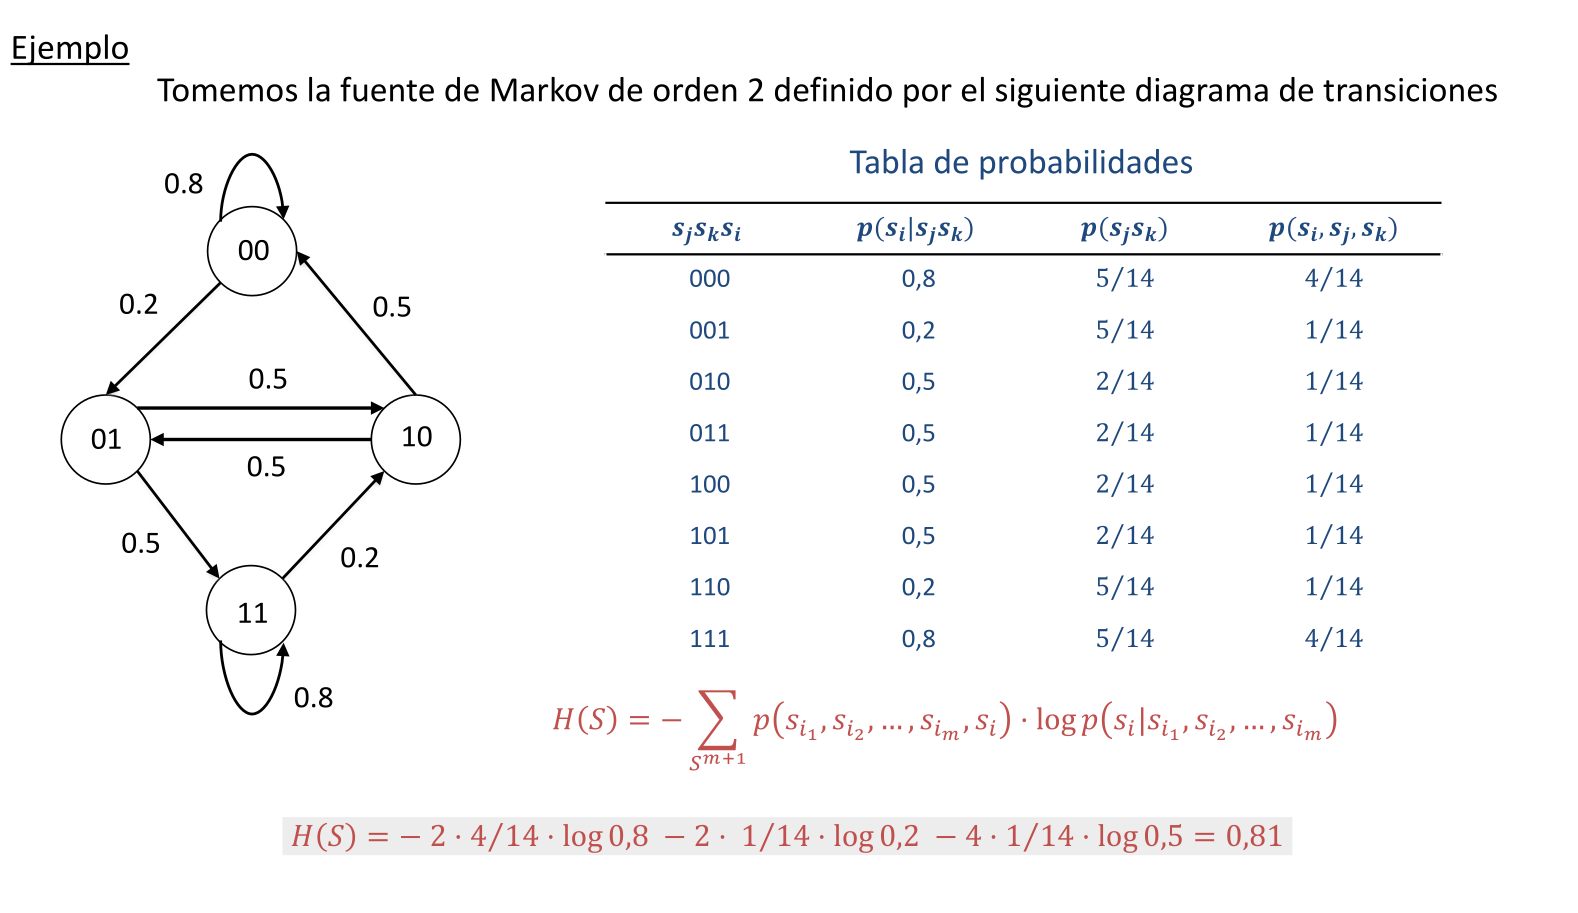
\includegraphics[width=0.9\textwidth]{entropia_markov.png}
   \caption{Ejemplo de cálculo de entropía a partir de una Fuente de Markov.}
   \label{fig:etiqueta_opcional}
\end{figure}


Por lo tanto, en una fuente de Markov de orden m, la probabilidad de ocurrencia de un símbolo, depende de los (m-1) símbolos anteriores. Cuanto mayor sea el orden (m), más información del contexto de incluye, y, en consecuencia, menores valores de entropía. Esto significa que modificar los valores de m, puede revelar patrones o regiones funcionales dentro de la secuencia dada. 

\chapter{Metodología}


\section{Material y herramientas}

\subsection{Entorno de Trabajo}

El entorno de desarrollo se basa en el sistema operativo Linux, ya que muchas de las bibliotecas necesarias para el análisis de archivos VCF, como vcfpy, no tienen soporte en Windows. Para ello, se utiliza:
\begin{itemize}
   \item WSL (Windows Subsystem for Linux) en máquinas con sistema Windows.
   \item Ubuntu directamente instalado en el equipo de trabajo de la oficina.
\end{itemize}

Como gestor de entornos y dependencias se emplea Anaconda, una distribución de Python orientada a ciencia de datos, bioinformática y aprendizaje automático. Anaconda incluye numerosas librerías útiles como numpy, pandas, matplotlib, scikit-learn, entre otras, y permite la creación de entornos virtuales aislados.

\subsection{Archivos necesarios}

\subsubsection{Archivos FASTA}

El archivo FASTA es un formato estándar utilizado para almacenar secuencias de ADN, ARN o proteínas. Este formato de texto simple presenta las secuencias de interés precedidas por una línea de cabecera que comienza con el carácter > seguido de un identificador o descripción de la secuencia. 

En el presente trabajo, los archivos FASTA utilizados deben corresponder al ensamblaje genómico GRCh37.p13, disponible en la base de datos NCBI (National Center for Biotechnology Information). Cada archivo FASTA corresponde a un cromosoma específico de los 46 cromosomas principales del genoma humano. 

Se ha realizado mediante descarga local de estos archivos, ya que el acceso directo a las secuencias mediante peticiones a NCBI puede generar errores por limitaciones de memoria RAM en la ejecución del programa. 

\subsubsection{Archivos VCF}

El formato VCF (Variant Call Format) es un tipo de archivo utilizado para almacenar variantes genómicas identificadas. De aquí nos interesan especialmente: 

\begin{itemize}
   \item Líneas de metainformación. 
   \item Una línea de encabezado.
   \item Líneas de datos, donde cada línea describe una variante concreta. 
\end{itemize}

Cada variante contiene información sobre la posición en el genoma, el cromosoma, la base de referencia, la base alternativa, así como otros datos asociados a la calidad y características de la variante. De los tipos de variantes estudiados en la sección de fundamentos, los presentes en el archivo VCF con el que trabajamos son los siguientes: 

\begin{itemize}
   \item SNPs (Single Nucleotide Polymorphisms). 
   \item Inserciones. 
   \item Deleciones.
\end{itemize}

Por último, de los archivos VCF extraeremos la siguiente información esencial: 

\begin{itemize}
   \item Cromosoma en el que se encuentra la variante.
   \item Posición de la variante dentro del cromosoma.  
   \item Base de la secuencia de referencia.
   \item Base correspondiente a la secuencia mutada.
\end{itemize}
 

\subsection{Librería utilizadas}

Durante el desarrollo de este TFG, ha sido necesario apoyarse en algunas herramientas que requerían la instalación de ciertas librerías presentes para Python, tanto para el procesamiento y análisis del genoma como para la visualización de los distintos gráficos y el desarrollo de la interfaz de usuario. A continuación, se describen las principales librerías utilizadas y su aportación al proyecto:

\begin{itemize}
   \item Bio (biopython) es la librería por excelencia para la bioinformática, utilizada para acceder a las bases de datos del NCBI (mediante BIO.Entrez), y para la lectura y análisis de los archivos que contienen las secuencias genómicas en formato FASTA (mediante Bio.SeqIO).
   \item Vcfpy es una librería creada para Python 3, y especializada en el manejo de archivos VCF. Esta permite leer, analizar y escribir los archivos con mutaciones de manera estructurada en computacionalmente eficiente, y extraer de manera sencilla e intuitiva la información que se requiere.
   \item Matplotlib es una de las librerías más utilizadas de Python, y se encarga de la generación de gráficos. En este caso se emplea para visualizar de manera clara tres listas: la entropía simple, la entropía generada a partir de Fuentes de Markov, y la densidad de mutaciones en la secuencia genómica. Además, se ha configurado un backend (TkAgg) para poder trabajar sin interfaz gráfica, de manera que genera imágenes exportables (en formato png). Por último, se hace uso de matplotlib.ticker, que es un módulo auxiliar que permite personalizar los ejes y formatos numéricos en los gráficos generados.
   \item Pandas es una librería para el análisis y manipulación de datos en forma de tablas, que se utiliza para gestionar y mostrar la información extraída de los archivos VCF y almacenar resultados intermedios, como mutaciones no aplicadas.
   \item Numpy es la biblioteca utilizada para lograr la optimización en los cálculos numéricos. En este contexto se usa para operaciones como el cálculo de la entropía de Shannon y la entropía basada en modelos de Markov, ya que permite manejar grandes volúmenes de datos genómicos de forma eficiente.
   \item Streamlit es una librería de Python de código abierto que facilita la creación y el intercambio de aplicaciones web para la ciencia de datos y el machine learning. Es una forma rápida y sencilla de convertir código Python en una aplicación web interactiva, sin necesidad de conocimientos previos de desarrollo web . En este proyecto, Streamlit facilita al usuario la carga de archivos VCF, la selección del cromosoma de estudio y la visualización de resultados gráficos y tabulares, sin necesidad de conocimientos técnicos avanzados.
\end{itemize}


\section{Hipótesis}

La hipótesis de partida se basa en la idea de que la entropía de una secuencia de ADN experimenta cambios significativos en las regiones donde puede haber mutaciones patogénicas. Estas regiones de valores anómalos entropía podrían coincidir con las zonas funcionales asociadas a enfermedades raras. 

El análisis se estructura en tres casos de estudio diferentes, cada uno enfocado a detectar patrones distintos en la secuencia:

\subsection{Caso 1: Cálculo de entropía en ventanas deslizantes}

En este primer análisis, se calcula la entropía en ventanas deslizantes de tamaño w a lo largo de la secuencia genómica. El objetivo es comparar las variaciones de entropía entre la secuencia de referencia y la secuencia mutada.

La entropía $H$ para cada ventana se calcula como:

\[
H = - \sum p(kmer) \cdot \log_2 p(kmer)
\]

Donde:

\begin{itemize}
   \item $p(kmer)$ es la probabilidad de aparición de un k-mer dentro de la ventana.
   \item La probabilidad se calcula como la fracción de la frecuencia de ese k-mer entre el número de tipos distintos de k-mer en la ventana.
\end{itemize}

Se recorren ambas secuencias (referencia y mutada) y se calcula la entropía de cada ventana. Posteriormente, se representan gráficamente las entropías de ambas secuencias a lo largo de la posición genómica para detectar picos o variaciones significativas.


\subsection{Caso 2: Cálculo de densidad de mutaciones}

En este segundo análisis, se estudia la densidad de mutaciones presentes en las regiones cercanas a cada variante detectada en el archivo VCF.

Para ello, se toma una ventana de tamaño 2L centrada en cada mutación, es decir, se consideran L posiciones antes y L posiciones después de la posición de la mutación. Dentro de esta ventana, se cuenta el número de mutaciones existentes. Este procedimiento se repite para cada mutación presente en el archivo VCF.

El resultado se almacena en una lista que posteriormente se utiliza para generar un gráfico de densidad de mutaciones. Este gráfico representa las zonas con mayor concentración de variantes, lo cual podría indicar regiones funcionales afectadas.


\subsection{Caso 3: Cálculo de entropía basada en probabilidades condicionales (Modelo de Markov)}

En el tercer análisis, se utiliza un enfoque más avanzado basado en modelos de Markov de orden k para calcular la entropía condicional entre k-mers.

\subsubsection{Creación del Autómata}

Se construye un autómata que permite modelar la secuencia como una cadena de
estados, donde:

\begin{itemize}
   \item El alfabeto está formado los diferentes nucletidos {A, C, G, T}.
   \item Los estados iniciales se corresponden con los primeros caracteres de los k-mers.
   \item Los estados finales corresponden a los últimos caracteres de cada k-mer.
   \item Las transiciones representan la concatenación de bases adyacentes.
\end{itemize}


Por ejemplo, dado un conjunto de k-mers {ACGT, ACCD}, se define:

\begin{itemize}
   \item Alfabeto: {A, C, G, T, D}.
   \item Estados iniciales: {A}.
   \item Estados finales: {T, D}.
   \item Transiciones: {AC, CG, GT, CC, CD} (para un modelo de segundo orden).
\end{itemize}


\subsubsection{Cálculo de Probabilidades de Transición}
Una vez definido el autómata, se recorren las secuencias y se cuentan las ocurrencias de cada transición. Con esta información, se calcula la probabilidad de transición desde un estado s a otro estado t como:

\[
p(s \to t) = \frac{\text{Número de transiciones de } s \to t}{\text{Total de transiciones desde } s}
\]

Si una transición no existe, se le asigna una probabilidad muy baja para evitar problemas en el cálculo del logaritmo.

\subsubsection{Cálculo de Entropía Condicional}

Se desliza una ventana de tamaño w sobre la secuencia y, dentro de esta ventana, se analizan las transiciones de tamaño k para calcular la contribución a la entropía condicional de cada transición.

La entropía total de la ventana se calcula restando las contribuciones de todas las transiciones observadas.


\chapter{Desarrollo}

\section{Importación de librerías y configuración inicial }

En primer lugar, se realizan importaciones de librerías necesarias para ejecutar distintas funciones en el análisis genómico y se realiza una configuración inicial del servidor de Streamlit. 

En back.py, el archivo que contiene la lógica de la aplicación, se hace uso de diversas bibliotecas necesarias para recuperar secuencias genómicas, analizarlas, generar gráficos, y trabajar con datos genómicos en diversos formatos. Se usan módulos estándar como math y time, y otros especializados como matplotlib para generar gráficos (aunque configurado para un backend sin interfaz gráfica con TkAgg), pandas y numpy para análisis de datos, y Bio de Biopython para acceder a bases de datos biológicas del NCBI. También se importa vcfpy para manejar archivos VCF (usados en genómica para representar variantes), y requests para hacer solicitudes HTTP. 

En interfaz.py, se importan los módulos necesarios para construir la interfaz web con Streamlit, la herramienta de Python para crear aplicaciones interactivas. Se importa st de streamlit para generar la UI, AnalizadorGenomico desde el archivo back.py (que contiene la lógica), y bibliotecas estándar como pandas para manejo de datos, os para operaciones del sistema de archivos, y zipfile para comprimir archivos.  

Adicionalmente, se ha añadido el archivo config.toml en la carpeta streamlit, estableciendo el parámetro maxUploadSize = 1000 dentro de la sección [server]. Esto significa que se ha aumentado el límite máximo de tamaño de archivo que el usuario puede subir a la aplicación a 1 GB, lo cual es necesario para poder trabajar con archivos genómicos grandes como las secuencias genómicas o los VCFs. 


\section{Lectura de las mutaciones presentes en el archivo VCF}

En segundo lugar, se realiza la lectura del archivo VCF correspondiente a los pacientes que presentan una determinada enfermedad rara (en este caso retinosis pigmentaria). 

Para ello, se utiliza una librería específica de Python (vcfpy), que permite extraer de manera estructurada los datos contenidos en el archivo. El programa recorre cada línea del VCF (ignorando las líneas de encabezado) y obtiene los datos fundamentales de cada mutación. Sin embargo, no necesitamos obtener los detalles de todas las mutaciones, por lo que se realiza un filtrado para obtener solo las mutaciones que se encuentren en el cromosoma especificado por el usuario. 


\section{Almacenamiento de las mutaciones en una estructura de datos adecuada}

Una vez extraídas las mutaciones del archivo VCF, se almacenan en un diccionario de Python (ya que permite un acceso rápido y una organización estructurada y eficiente), de tal manera que cada mutación queda registrada mediante los siguientes campos: 

\begin{itemize}
   \item Cromosoma en el que se encuentra la variante.
   \item Posición exacta dentro del cromosoma.
   \item Base de la secuencia de referencia.
   \item Base correspondiente a la secuencia mutada.
\end{itemize}

\section{Extracción de la secuencia de referencia del cromosoma correspondiente}

En este paso, se procede a la lectura del archivo FASTA que contiene la secuencia de referencia del cromosoma que se desea analizar.  

Debido a que la secuencia de un cromosoma entero contiene una cantidad de información extremadamente elevada, su procesamiento sería muy costoso computacionalmente. Además, la generación de gráficos de toda la secuencia sería demasiado compleja. Por lo tanto, se ha optado por procesar la secuencia en bloques más pequeños, permitiendo un análisis más eficiente y visualmente interpretable. 

Este archivo se abre en modo lectura (with open(fasta\_file, ``r'') as file) y se recorre línea a línea.

Para comprobar que el número de cromosoma es correcto, se limpia la cabecera eliminando el símbolo >\ y cualquier espacio extra, tomando solo el primer fragmento del ID en caso de que haya espacios (por ejemplo, si el encabezado es ``chr1\dots info'', se queda solo con ``chr1''). Si el id del registro coincide con el cromosoma solicitado por el usuario, se extrae la secuencia en el rango especificado y se convierte a mayúsculas. 

Una vez extraída la secuencia, se han considerado dos opciones en caso de que la secuencia contenga caracteres N (indicando zonas donde no se conoce con certeza la base presente): 

1. estas posiciones serán ignoradas y no se tendrán en cuenta en los cálculos de entropía o en el análisis de las mutaciones, ya que no aportan información relevante, 

2. serán tratadas como un nuevo tipo de base nitrogenada, entendiendo que también aportan información a los valores de la entropía. 

En cualquier caso, estas zonas desconocidas no están cerca de ninguna mutación con las que se está trabajando, por lo que no es relevante el tratamiento que se les dé. 

\section{Aplicación de las mutaciones sobre la secuencia de referencia}

Una vez obtenida la secuencia de referencia del cromosoma, se incorporan las mutaciones almacenadas previamente. Para ello, el primer paso es convertir la secuencia de referencia en una lista para permitir la modificación directa de esta. 

Después, se extraen solo las mutaciones correspondientes al cromosoma actual y se ordenan por posición. Para cada mutación, se ajusta la posición relativa dentro de la secuencia, ya que debemos considerar los posibles desplazamientos por cambios de longitud en mutaciones anteriores (por ejemplo, AAT --> A). Se extrae el segmento de referencia de la secuencia y se compara con la mutación esperada: se comprueba que las bases presentes en la posición correspondiente de la secuencia de referencia coinciden con las bases de referencia indicadas en el archivo VCF. 

En caso de que esta base coincida, se aplica la mutación, reemplazando el fragmento correspondiente con la nueva variante y se actualiza el desplazamiento, para ajustar futuras posiciones si cambia la longitud. 

En cambio, si la base no coincide (posible error en los datos o desactualización del archivo FASTA), la mutación se descarta, se almacena la información de dicha mutación en un archivo para su posterior análisis o revisión y se imprime una advertencia. 

Este proceso da lugar a una nueva secuencia mutada, sobre la cual se realizarán las comparaciones con la secuencia original. 

\section{Cálculo de la entropía mediante ventanas deslizantes}

A continuación, se calcula la entropía simple sobre ambas secuencias (referencia y mutada) utilizando una ventana deslizante de tamaño w (w > k). 

Para ello se define primero una función para contar la frecuencia de cada k-mer en la secuencia (subcadenas de longitud k). Esto se realiza recorriendo la secuencia, extrayendo cada subcadena de longitud k e introduciéndola en un diccionario donde las claves son los k-mers y los valores son las frecuencias (se suma 1 por cada aparición a la entrada correspondiente).  

Después, se procede a calcular la entropía de Shannon en ventanas deslizantes de tamaño w sobre la secuencia, basada en la distribución de k-mers dentro de cada ventana. La ventana se desplaza a lo largo de la secuencia en pasos de una posición, y dentro de cada ventana se calcula la entropía en base a las probabilidades de aparición de cada k-mer con la siguiente fórmula: 

$H = -\sum p_i \cdot \log_2(p_i)$, donde $p_i$ es la probabilidad del k-mer $i$.

Una vez calculada, se añade la entropía a una lista, y finalmente se devuelve la lista de entropías de cada ventana. 

\section{Representación gráfica de la entropía en ambas secuencias}

Una vez obtenida la lista de entropías de ambas secuencias, se procede a su representación gráfica mediante librerías de visualización de Python (matplotlib). 

Los gráficos permiten observar de forma clara las zonas de la secuencia en las que se produce un incremento o decremento significativo de la entropía debido a la presencia de mutaciones. 

Estos cambios podrían estar asociados a regiones funcionales relevantes en el genoma o a zonas afectadas por enfermedades. 

\section{Cálculo de la densidad de mutaciones}

En este paso, se analiza la concentración de mutaciones en torno a cada variante presente en el archivo VCF. 

Para ello, se centra una ventana de tamaño 2L en cada mutación, considerando L posiciones hacia atrás y L posiciones hacia adelante desde la posición de la variante. 

Dentro de esta ventana, se cuenta el número total de mutaciones presentes, y se guarda en una tupla (pos, cuenta) indicando cuántas mutaciones hay en torno a pos. Este procedimiento se repite para todas las mutaciones del cromosoma, generando una lista de valores que reflejan la densidad de mutaciones en distintas regiones. 

\section{Representación gráfica de la densidad de mutaciones}

La lista obtenida en el paso anterior se utiliza para generar un gráfico que permite visualizar las regiones con mayor concentración de variantes.

Este tipo de representación la utilizamos para detectar zonas del genoma donde se acumulan un elevado número de mutaciones, las cuales están resaltadas y se especifican sus valores concretos.

\section{Construcción del autómata para el cálculo de probabilidades de transición}

En este paso se construye un autómata basado en un modelo de Markov de orden K (no confundir con el parámetro k de los k-mers), con el objetivo de modelar las transiciones entre k-mers presentes en la secuencia. 

Para ello, primero se define un alfabeto formado por las diferentes bases {A, C, G, T} y se recorre la secuencia para generar los estados del autómata, definidos por subcadenas de longitud K - 1, y se registran las transiciones entre dichos estados como el paso de un estado a otro adyacente, desplazado en una base. Además, se obtienen los estados iniciales y finales a partir de los k-mers, que son aquellos estados que constituyen el comienzo y final, respectivamente, de un k-mer.  

Una vez construido el autómata, se recorren las secuencias analizadas y se calculan las probabilidades de transición entre estados dividiendo la frecuencia de cada transición entre el total de transiciones posibles desde su estado origen. El resultado final es un autómata que consiste en cuatro elementos:  


\begin{itemize}
   \item El alfabeto de símbolos.
   \item El conjunto de estados iniciales.  
   \item El conjunto de estados finales. 
   \item La matriz de transición probabilística de los estados 
\end{itemize}

\section{Representación y guardado del autómata}

Una vez construido el autómata, se procede a su representación mediante guardado de los elementos principales en formato texto en un archivo txt. Se genera un archivo para la secuencia original y otro para la secuencia mutada para poder realizar comparaciones. 

En este archivo se representan los elementos principales de la siguiente manera: 

\begin{itemize}
   \item Alfabeto como una lista con las diferentes bases nitrogenadas 
   \item Estados iniciales y finales, como una lista de secuencias de tamaño K-1.
   \item Transiciones, como una lista de tuplas del tipo: (estado actual, símbolo, siguiente estado)
\end{itemize}


\section{Cálculo de las probabilidades de transición y de la entropía condicional}

A partir de las probabilidades almacenadas en el autómata, se calcula la entropía condicional dentro de ventanas deslizantes de tamaño w, teniendo en cuenta las transiciones presentes en cada ventana. 

Para ello, primero se recorre la secuencia usando una ventana deslizante de tamaño w, extrayendo una subsecuencia en cada iteración y dentro de cada ventana, se recorre la subsecuencia formando pares de estado actual, siguiente estado para obtener el valor de la probabilidad para esa transición. Ahora se aplica la fórmula de la entropía sumando el valor negativo de $p \cdot \log_2(p)$ para cada transición (si la transición no se encuentra, se asume una probabilidad muy pequeña para evitar $\log(0)$).


Esto permite obtener una medida de la entropía, considerando no solo la frecuencia de k-mers individuales, sino también las relaciones de dependencia entre bases. 

\section{Interfaz gráfica}

Finalmente, con el objetivo de facilitar el uso de esta aplicación a usuarios no expertos en programación, se ha implementado una interfaz gráfica utilizando la biblioteca Streamlit, una herramienta en Python que permite construir aplicaciones web interactivas de forma sencilla y eficiente. 

Esta interfaz permite realizar análisis genómicos de manera accesible y guiada a través de los diferentes pasos necesarios para cargar los datos, configurar los parámetros de análisis, ejecutar el procesamiento y visualizar o descargar los resultados generados. 

 

A través de esta interfaz, el usuario podrá introducir una serie de parámetros entre los que se incluyen:  


\begin{itemize}
   \item Seleccionar el número de cromosoma a analizar desde un menú desplegable. A partir de esta selección, el sistema asocia automáticamente el identificador del cromosoma en formato GRCh37 y el archivo FASTA correspondiente (en caso de que no se encuentre, se muestra un mensaje de error). 
   \item Se debe proporcionar un archivo con las mutaciones del paciente en formato VCF, cargado a través de subida de archivos. 
   \item Tamaño de k-mer ($k$), que define el tamaño de las secuencias. 
    \item Orden del modelo de Markov ($k_{\text{markov}}$), que determina cuántos símbolos anteriores se consideran en la probabilidad condicional.
    \item Tamaño de ventana para densidad ($l$), que establece el rango en el que se tienen en cuenta las mutaciones alrededor de cada variante. 
    \item Tamaño de ventana para entropía ($w$), para el cálculo de las entropías.
   \item Posición de inicio y tamaño del bloque, para definir el segmento del cromosoma a analizar y así no cargar regiones genómicas excesivamente grandes. 
\end{itemize}


 

Una vez introducidos estos datos, la aplicación se encarga de ejecutar la lógica del programa: aplica las mutaciones del archivo VCF sobre la secuencia original, calcula la entropía simple y la entropía basada en probabilidades condicionales, analiza la densidad de mutaciones en regiones del genoma y genera los gráficos y archivos correspondientes. Finalizado este análisis, se devuelven las siguientes salidas:  

\begin{itemize}
   \item Tres imágenes descargables con los gráficos de entropía simple, entropía condicional (o de Markov) y densidad de mutaciones. 
   \item Tres archivos para descargar: dos ficheros de texto con los autómatas de la secuencia original y secuencia mutada (los generados a partir de Fuentes de Markov), y un archivo con las mutaciones que no han podido aplicarse. 
   \item Además, se proporciona la opción de descargar un archivo comprimido (.zip) que incluye todos los resultados para facilitar su almacenamiento o distribución. 
\end{itemize}
 



\chapter{Experimentos}

????? ????????????? ????????????? ????????????? ????????????? ????????????? 

\section{?? ???? ???? ? ?? ??}

????? ????????????? ????????????? ????????????? ????????????? ?????????????

%%%%%%%%%%%%%%%%%%%%%%%%%%%%%%%%%%%%%%%%%%%%%%%%%%%%%%%%%%%%%%%%%%%%%%%%%%%%%%%
%                                 CONCLUSIONS                                 %
%%%%%%%%%%%%%%%%%%%%%%%%%%%%%%%%%%%%%%%%%%%%%%%%%%%%%%%%%%%%%%%%%%%%%%%%%%%%%%%

\chapter{Conclusiones}

????? ????????????? ????????????? ????????????? ????????????? ????????????? 

%%%%%%%%%%%%%%%%%%%%%%%%%%%%%%%%%%%%%%%%%%%%%%%%%%%%%%%%%%%%%%%%%%%%%%%%%%%%%%%
%                                BIBLIOGRAFIA                                 %
%%%%%%%%%%%%%%%%%%%%%%%%%%%%%%%%%%%%%%%%%%%%%%%%%%%%%%%%%%%%%%%%%%%%%%%%%%%%%%%

\begin{thebibliography}{99}

%%%%%%%%%%%%%%%%%%%%%%%%%%%%%%%%%%%%%%%%%%%%%%%%%%%%%%%%%%%%%%%%%%%%%%%%%%%%%%%
% MODEL D'ARTICLE                                                             %
%%%%%%%%%%%%%%%%%%%%%%%%%%%%%%%%%%%%%%%%%%%%%%%%%%%%%%%%%%%%%%%%%%%%%%%%%%%%%%%
\bibitem{light}
   Jennifer~S. Light.
   \newblock When computers were women.
   \newblock \textit{Technology and Culture}, 40:3:455--483, juliol, 1999.

\bibitem{fuentesupv}
   Departamento de Lenguajes y Sistemas Informáticos.
   \newblock \textit{Fuentes de Información}.
   \newblock Universitat Politècnica de València, versión 2, s.f.
   
%%%%%%%%%%%%%%%%%%%%%%%%%%%%%%%%%%%%%%%%%%%%%%%%%%%%%%%%%%%%%%%%%%%%%%%%%%%%%%%
% MODEL DE LLIBRE                                                             %
%%%%%%%%%%%%%%%%%%%%%%%%%%%%%%%%%%%%%%%%%%%%%%%%%%%%%%%%%%%%%%%%%%%%%%%%%%%%%%%
\bibitem{ifrah}
   Georges Ifrah.
   \newblock \textit{Historia universal de las cifras}.
   \newblock Espasa Calpe, S.A., Madrid, sisena edició, 2008.

\bibitem{COV}
   Thomas M. Cover and Joy A. Thomas.  
   \newblock \textit{Elements of Information Theory}.  
   \newblock Wiley-Interscience, segunda edición, 2006.

\bibitem{WAT}
   J.~D.~Watson, T.~A.~Baker, S.~P.~Bell, A.~Gann, M.~Levine i R.~Losick.
   \newblock \textit{Molecular Biology of the Gene}.
   \newblock Pearson Education, 7a edició, 2013.

%%%%%%%%%%%%%%%%%%%%%%%%%%%%%%%%%%%%%%%%%%%%%%%%%%%%%%%%%%%%%%%%%%%%%%%%%%%%%%%
% MODEL D'URL                                                                 %
%%%%%%%%%%%%%%%%%%%%%%%%%%%%%%%%%%%%%%%%%%%%%%%%%%%%%%%%%%%%%%%%%%%%%%%%%%%%%%%

\bibitem{NAT}
   National Eye Institute.  
   \newblock Retinitis pigmentaria | National Eye Institute.  
   \newblock Disponible en  
   \url{https://www.nei.nih.gov/espanol/aprenda-sobre-la-salud-ocular/enfermedades-y-afecciones-de-los-ojos/retinitis-pigmentaria}.

\bibitem{GIL}
   Gil, G. A., Checa, F. L., Borrego, S., Chaparro-Hernández, P., Rueda, T. R., y Sanchez, J.  
   \newblock Estudio de la variabilidad clínica y la heterogeneidad genética en la retinitis pigmentosa.  
   \newblock Dialnet, 1994.    
   \newblock Disponible en  
   \url{https://dialnet.unirioja.es/servlet/articulo?codigo=6768158}.

\bibitem{STO}
   Stone, E. M.  
   \newblock Genetic Testing for Inherited Eye Disease.  
   \newblock \textit{Archives of Ophthalmology}, 125(2):205, 2007.  
   \newblock Disponible en
   \newblock \url{https://doi.org/10.1001/archopht.125.2.205}.

\bibitem{HAN}
   Hanany, M., Rivolta, C., \& Sharon, D.  
   \newblock Worldwide carrier frequency and genetic prevalence of autosomal recessive inherited retinal diseases.  
   \newblock \textit{Proceedings of the National Academy of Sciences}, 117(5):2710–2716, 2020.  
   \newblock Disponible en
   \newblock \url{https://doi.org/10.1073/pnas.1913179117}.

\bibitem{DEC}
   De Castro Miró, M.  
   \newblock \textit{Diagnóstico genético de las distrofias hereditarias de retina mediante secuenciación masiva de nueva generación (NGS)}.  
   \newblock Tesis doctoral, Universitat de València, 2017.  
   \newblock Repositorio UV.  
   \newblock Disponible en
   \newblock \url{https://roderic.uv.es/handle/10550/61138}.

\bibitem{SHE}
   Shen, D., Wu, G., \& Suk, H.
   \newblock Deep Learning in Medical Image Analysis.
   \newblock \textit{Annual Review of Biomedical Engineering}, 19(1), 221--248, 2017.
   \newblock Disponible en
   \newblock \url{https://doi.org/10.1146/annurev-bioeng-071516-044442}

\bibitem{VER}
   Verana Health.  
   \newblock Why Real-World Data is Key to Providing Insights Into Retinitis Pigmentosa,  
   emés el 20 de novembre de 2024.  
   \newblock Disponible en  
   \url{https://veranahealth.com/why-real-world-data-is-key-to-providing-insights-into-retinitis-pigmentosa/}.

\bibitem{HAR}
   Hartong, D. T., Berson, E. L., \& Dryja, T. P.  
   \newblock Retinitis pigmentosa.  
   \newblock \textit{The Lancet}, vol. 368, núm. 9549, pp. 1795--1809, 2006.  
   \newblock Disponible en  
   \url{https://doi.org/10.1016/s0140-6736(06)69740-7}.

\bibitem{FER}
   Ferreira, H., Marta, A., Machado, J., Couto, I., Marques, J. P., Beirão, J. M., \& Cunha, A.  
   \newblock Retinitis Pigmentosa Classification with Deep Learning and Integrated Gradients Analysis.  
   \newblock \textit{Applied Sciences}, vol. 15, núm. 4, art. 2181, 2025.  
   \newblock Disponible en  
   \url{https://doi.org/10.3390/app15042181}.

\bibitem{STE}
   Stevenson, S.  
   \newblock How deep learning may play a role in predicting retinitis pigmentosa visual impairment,  
   emés el 14 de març de 2023.  
   \newblock Disponible en  
   \url{https://www.ophthalmologytimes.com/view/how-deep-learning-may-play-a-role-in-predicting-retinitis-pigmentosa-visual-impairment}.

\bibitem{ISS}
   Issa, Mohamad et al.  
   \newblock Applications of artificial intelligence to inherited retinal diseases: A systematic review.  
   \newblock \textit{Survey of Ophthalmology}, vol. 70, núm. 2, pp. 255--264.  

\bibitem{SEC}
   Societat Espanyola de Ciències de la Computació i Llenguatges (SECal).  
   \newblock Aplicaciones de la Teoría de la Información en Genómica,  
   sense data.  
   \newblock Disponible en  
   \url{https://www.secal.es}.

\bibitem{VOZ}
   N.D.  
   \newblock Un algoritmo encuentra indicios de enfermedades en la parte del ADN que teóricamente no servía para nada,  
   emés el 21 d’abril de 2025.  
   \newblock Disponible en  
   \url{https://media.lavozdegalicia.es/noticia/sociedad/2025/04/21/algoritmo-encuentra-indicios-enfermedades-parte-adnconsidera-inutil/00031745236367256507381.htm}.

\bibitem{WAN}
   Wang, Y., Juroch, K., Chen, Y., Ying, G., \& Birch, D. G.  
   \newblock Deep Learning–Facilitated Study of the Rate of Change in Photoreceptor Outer Segment Metrics in RPGR-Related X-Linked Retinitis Pigmentosa.  
   \newblock \textit{Investigative Ophthalmology \& Visual Science}, vol. 64, núm. 14, art. 31, 2023.  
   \newblock Disponible en  
   \url{https://doi.org/10.1167/iovs.64.14.31}.

\bibitem{ZON}
   ZonaIT.  
   \newblock Avances en la terapia génica para la retinosis pigmentaria causada por mutaciones en el gen RPGR,  
   sense data.  
   \newblock Disponible en  
   \url{https://biotech-spain.com/es/articles/avances-en-la-terapia-g-nica-para-la-retinosis-pigmentaria-causada-por-mutaciones-en-el-gen-rpgr}.

\bibitem{ZHA}
   F.~Zhang, W.~Gu, M.~E.~Hurles, i J.~R.~Lupski.
   \newblock Copy Number Variation in Human Health, Disease, and Evolution.
   \newblock \textit{Annual Review of Genomics and Human Genetics}, 10(1):451--481, 2009.
   \newblock Disponible en
   \newblock \url{https://doi.org/10.1146/annurev.genom.9.081307.164217}.
   
\bibitem{JAV}
   Javier, A.  
   \newblock ¿Qué es el formato FASTA?    
   \newblock Disponible en 
   \newblock \url{https://es.scribd.com/document/540407009/que-es-el-formato-fasta}
 
\bibitem{FAS}
   National Center for Biotechnology Information (NCBI).  
   \newblock FASTA Format for Nucleotide Sequences. 
   \newblock Disponible en 
   \newblock \url{https://www.ncbi.nlm.nih.gov/genbank/fastaformat/}
 
\bibitem{AUT}
   Auton, A., Abecasis, G. R., Altshuler, D. M., Durbin, R. M., Bentley, D. R., Chakravarti, A., Clark, A. G., Donnelly, P., Eichler, E. E., Flicek, P., Gabriel, S. B., Gibbs, R. A., Green, E. D., Hurles, M. E., Knoppers, B. M., Korbel, J. O., Lander, E. S., Lee, C., et al.  
   \newblock A global reference for human genetic variation.  
   \newblock \textit{Nature}, 526(7571), 68–74, 2015.  
   \newblock Disponible en 
   \newblock \url{https://doi.org/10.1038/nature15393}
   
\bibitem{GEN}
   National Human Genome Research Institute (NHGRI).  
   \newblock Introduction to Genomics.  
   \newblock Disponible en  
   \newblock \url{https://www.genome.gov/About-Genomics/Introduction-to-Genomics}


\bibitem{EMB}
   EMBL-EBI.  
   \newblock Understanding VCF format | Human genetic variation.  
   \newblock Disponible en 
   \newblock \url{https://www-ebi-ac-uk.translate.goog/training/online/courses/human-genetic-variation-introduction/variant-identification-and-analysis/understanding-vcf-format/?_x_tr_sl=en&_x_tr_tl=es&_x_tr_hl=es&_x_tr_pto=sge}
   
\bibitem{DAN}
   Danecek, P., Auton, A., Abecasis, G., Albers, C. A., Banks, E., DePristo, M. A., Handsaker, R. E., Lunter, G., Marth, G. T., Sherry, S. T., McVean, G., \& Durbin, R.  
   \newblock The variant call format and VCFtools.  
   \newblock \textit{Bioinformatics}, 27(15), 2156–2158, 2011.  
   \newblock \url{https://doi.org/10.1093/bioinformatics/btr330}

\bibitem{GEN}
   Genómica computacional.  
   \newblock Formato FASTA.  
   \newblock \textit{Google Sites}, consultado en mayo de 2025.  
   \newblock Disponible en: \url{https://sites.google.com/site/genomicaciencias/laboratorio/formato-fasta}

\bibitem{RIN}
   J.~L.~Rinn i H.~Y.~Chang.
   \newblock Genome regulation by long noncoding RNAs.
   \newblock \textit{Annual Review of Biochemistry}, 81:145--166, 2012.
   \newblock Disponible en
   \newblock \url{https://doi.org/10.1146/annurev-biochem-051410-092902}

\bibitem{ROB}
   Roberto Togneri y Christopher J. S. deSilva.  
   \newblock \textit{Fundamentals of Information Theory and Coding Design}.  
   \newblock CRC Press, Boca Raton, Florida, 2006.
   

\end{thebibliography}
\cleardoublepage

%%%%%%%%%%%%%%%%%%%%%%%%%%%%%%%%%%%%%%%%%%%%%%%%%%%%%%%%%%%%%%%%%%%%%%%%%%%%%%%
%                           APÈNDIXS  (Si n'hi ha!)                           %
%%%%%%%%%%%%%%%%%%%%%%%%%%%%%%%%%%%%%%%%%%%%%%%%%%%%%%%%%%%%%%%%%%%%%%%%%%%%%%%

\APPENDIX

%%%%%%%%%%%%%%%%%%%%%%%%%%%%%%%%%%%%%%%%%%%%%%%%%%%%%%%%%%%%%%%%%%%%%%%%%%%%%%%
%                         LA CONFIGURACIO DEL SISTEMA                         %
%%%%%%%%%%%%%%%%%%%%%%%%%%%%%%%%%%%%%%%%%%%%%%%%%%%%%%%%%%%%%%%%%%%%%%%%%%%%%%%

\chapter{Configuració del sistema}

????? ????????????? ????????????? ????????????? ????????????? ?????????????

\section{Fase d'inicialització}

????? ????????????? ????????????? ????????????? ????????????? ?????????????

\section{Identificació de dispositius}

????? ????????????? ????????????? ????????????? ????????????? ?????????????

%%%%%%%%%%%%%%%%%%%%%%%%%%%%%%%%%%%%%%%%%%%%%%%%%%%%%%%%%%%%%%%%%%%%%%%%%%%%%%%
%                               ALTRES  APÈNDIXS                              %
%%%%%%%%%%%%%%%%%%%%%%%%%%%%%%%%%%%%%%%%%%%%%%%%%%%%%%%%%%%%%%%%%%%%%%%%%%%%%%%


\chapter{??? ???????????? ????}

????? ????????????? ????????????? ????????????? ????????????? ????????????? 



%%%%%%%%%%%%%%%%%%%%%%%%%%%%%%%%%%%%%%%%%%%%%%%%%%%%%%%%%%%%%%%%%%%%%%%%%%%%%%%
%                              FI DEL DOCUMENT                                %
%%%%%%%%%%%%%%%%%%%%%%%%%%%%%%%%%%%%%%%%%%%%%%%%%%%%%%%%%%%%%%%%%%%%%%%%%%%%%%%

\end{document}
